\section{Evaluation} \todo{Beide: Neu, echte Messungen einbauen}
Um unser Verfahren zur Richtungsbestimmung zu testen und die Genauigkeit zu bestimmen haben wir es in Simulation und Echtwelt evaluiert. Dabei haben wir die Abweichung der Richtungsbestimmung für verschiedene Richtungen und Frequenzen bestimmt.
\subsection{Simulation}
Zunächst haben wir unser Verfahren in der Simulation getestet, da diese automatisierte Tests ermöglicht und somit leicht sehr viele verschiedene Richtungen/Frequenzen getestet werden können. Dabei haben wir die Schallquellen für verschiedene Radien auf einer Kugeloberfläche positioniert. Der Tetraeder wurde mit $0.28m$ Kantenlänge simuliert, dies entspricht dem Tetraeder, den wir auch in der Echtwelt gebaut haben. Die Schallquellen wurden mit einer $500Hz$ Sinusschwingung simuliert.
\begin{figure}[H]
  \centering
  % GNUPLOT: LaTeX picture with Postscript
\begingroup
  \makeatletter
  \providecommand\color[2][]{%
    \GenericError{(gnuplot) \space\space\space\@spaces}{%
      Package color not loaded in conjunction with
      terminal option `colourtext'%
    }{See the gnuplot documentation for explanation.%
    }{Either use 'blacktext' in gnuplot or load the package
      color.sty in LaTeX.}%
    \renewcommand\color[2][]{}%
  }%
  \providecommand\includegraphics[2][]{%
    \GenericError{(gnuplot) \space\space\space\@spaces}{%
      Package graphicx or graphics not loaded%
    }{See the gnuplot documentation for explanation.%
    }{The gnuplot epslatex terminal needs graphicx.sty or graphics.sty.}%
    \renewcommand\includegraphics[2][]{}%
  }%
  \providecommand\rotatebox[2]{#2}%
  \@ifundefined{ifGPcolor}{%
    \newif\ifGPcolor
    \GPcolorfalse
  }{}%
  \@ifundefined{ifGPblacktext}{%
    \newif\ifGPblacktext
    \GPblacktexttrue
  }{}%
  % define a \g@addto@macro without @ in the name:
  \let\gplgaddtomacro\g@addto@macro
  % define empty templates for all commands taking text:
  \gdef\gplbacktext{}%
  \gdef\gplfronttext{}%
  \makeatother
  \ifGPblacktext
    % no textcolor at all
    \def\colorrgb#1{}%
    \def\colorgray#1{}%
  \else
    % gray or color?
    \ifGPcolor
      \def\colorrgb#1{\color[rgb]{#1}}%
      \def\colorgray#1{\color[gray]{#1}}%
      \expandafter\def\csname LTw\endcsname{\color{white}}%
      \expandafter\def\csname LTb\endcsname{\color{black}}%
      \expandafter\def\csname LTa\endcsname{\color{black}}%
      \expandafter\def\csname LT0\endcsname{\color[rgb]{1,0,0}}%
      \expandafter\def\csname LT1\endcsname{\color[rgb]{0,1,0}}%
      \expandafter\def\csname LT2\endcsname{\color[rgb]{0,0,1}}%
      \expandafter\def\csname LT3\endcsname{\color[rgb]{1,0,1}}%
      \expandafter\def\csname LT4\endcsname{\color[rgb]{0,1,1}}%
      \expandafter\def\csname LT5\endcsname{\color[rgb]{1,1,0}}%
      \expandafter\def\csname LT6\endcsname{\color[rgb]{0,0,0}}%
      \expandafter\def\csname LT7\endcsname{\color[rgb]{1,0.3,0}}%
      \expandafter\def\csname LT8\endcsname{\color[rgb]{0.5,0.5,0.5}}%
    \else
      % gray
      \def\colorrgb#1{\color{black}}%
      \def\colorgray#1{\color[gray]{#1}}%
      \expandafter\def\csname LTw\endcsname{\color{white}}%
      \expandafter\def\csname LTb\endcsname{\color{black}}%
      \expandafter\def\csname LTa\endcsname{\color{black}}%
      \expandafter\def\csname LT0\endcsname{\color{black}}%
      \expandafter\def\csname LT1\endcsname{\color{black}}%
      \expandafter\def\csname LT2\endcsname{\color{black}}%
      \expandafter\def\csname LT3\endcsname{\color{black}}%
      \expandafter\def\csname LT4\endcsname{\color{black}}%
      \expandafter\def\csname LT5\endcsname{\color{black}}%
      \expandafter\def\csname LT6\endcsname{\color{black}}%
      \expandafter\def\csname LT7\endcsname{\color{black}}%
      \expandafter\def\csname LT8\endcsname{\color{black}}%
    \fi
  \fi
    \setlength{\unitlength}{0.0500bp}%
    \ifx\gptboxheight\undefined%
      \newlength{\gptboxheight}%
      \newlength{\gptboxwidth}%
      \newsavebox{\gptboxtext}%
    \fi%
    \setlength{\fboxrule}{0.5pt}%
    \setlength{\fboxsep}{1pt}%
\begin{picture}(7200.00,5040.00)%
    \gplgaddtomacro\gplbacktext{%
      \colorrgb{0.50,0.50,0.50}%
      \put(942,1289){\makebox(0,0){\strut{}$-2$}}%
      \colorrgb{0.50,0.50,0.50}%
      \put(1347,1215){\makebox(0,0){\strut{}$-1.5$}}%
      \colorrgb{0.50,0.50,0.50}%
      \put(1752,1140){\makebox(0,0){\strut{}$-1$}}%
      \colorrgb{0.50,0.50,0.50}%
      \put(2157,1066){\makebox(0,0){\strut{}$-0.5$}}%
      \colorrgb{0.50,0.50,0.50}%
      \put(2562,992){\makebox(0,0){\strut{}$0$}}%
      \colorrgb{0.50,0.50,0.50}%
      \put(2966,918){\makebox(0,0){\strut{}$0.5$}}%
      \colorrgb{0.50,0.50,0.50}%
      \put(3371,843){\makebox(0,0){\strut{}$1$}}%
      \colorrgb{0.50,0.50,0.50}%
      \put(3775,769){\makebox(0,0){\strut{}$1.5$}}%
      \colorrgb{0.50,0.50,0.50}%
      \put(4180,695){\makebox(0,0){\strut{}$2$}}%
      \csname LTb\endcsname%
      \put(2198,830){\makebox(0,0){\strut{}x [m]}}%
      \colorrgb{0.50,0.50,0.50}%
      \put(4398,755){\makebox(0,0){\strut{}$-2$}}%
      \colorrgb{0.50,0.50,0.50}%
      \put(4606,870){\makebox(0,0){\strut{}$-1.5$}}%
      \colorrgb{0.50,0.50,0.50}%
      \put(4814,984){\makebox(0,0){\strut{}$-1$}}%
      \colorrgb{0.50,0.50,0.50}%
      \put(5022,1098){\makebox(0,0){\strut{}$-0.5$}}%
      \colorrgb{0.50,0.50,0.50}%
      \put(5229,1213){\makebox(0,0){\strut{}$0$}}%
      \colorrgb{0.50,0.50,0.50}%
      \put(5437,1327){\makebox(0,0){\strut{}$0.5$}}%
      \colorrgb{0.50,0.50,0.50}%
      \put(5645,1441){\makebox(0,0){\strut{}$1$}}%
      \colorrgb{0.50,0.50,0.50}%
      \put(5853,1556){\makebox(0,0){\strut{}$1.5$}}%
      \colorrgb{0.50,0.50,0.50}%
      \put(6061,1670){\makebox(0,0){\strut{}$2$}}%
      \colorrgb{0.50,0.50,0.50}%
      \put(6268,1784){\makebox(0,0){\strut{}$2.5$}}%
      \csname LTb\endcsname%
      \put(6029,1156){\makebox(0,0){\strut{}y [m]}}%
      \colorrgb{0.50,0.50,0.50}%
      \put(920,1384){\makebox(0,0)[r]{\strut{}$-2$}}%
      \colorrgb{0.50,0.50,0.50}%
      \put(920,1641){\makebox(0,0)[r]{\strut{}$-1.5$}}%
      \colorrgb{0.50,0.50,0.50}%
      \put(920,1899){\makebox(0,0)[r]{\strut{}$-1$}}%
      \colorrgb{0.50,0.50,0.50}%
      \put(920,2156){\makebox(0,0)[r]{\strut{}$-0.5$}}%
      \colorrgb{0.50,0.50,0.50}%
      \put(920,2413){\makebox(0,0)[r]{\strut{}$0$}}%
      \colorrgb{0.50,0.50,0.50}%
      \put(920,2669){\makebox(0,0)[r]{\strut{}$0.5$}}%
      \colorrgb{0.50,0.50,0.50}%
      \put(920,2926){\makebox(0,0)[r]{\strut{}$1$}}%
      \colorrgb{0.50,0.50,0.50}%
      \put(920,3184){\makebox(0,0)[r]{\strut{}$1.5$}}%
      \colorrgb{0.50,0.50,0.50}%
      \put(920,3441){\makebox(0,0)[r]{\strut{}$2$}}%
      \csname LTb\endcsname%
      \put(122,2413){\makebox(0,0){\strut{}z [m]}}%
    }%
    \gplgaddtomacro\gplfronttext{%
      \csname LTb\endcsname%
      \put(5236,4536){\makebox(0,0)[r]{\strut{}getestete Positionen (für 1.4m)}}%
    }%
    \gplbacktext
    \put(0,0){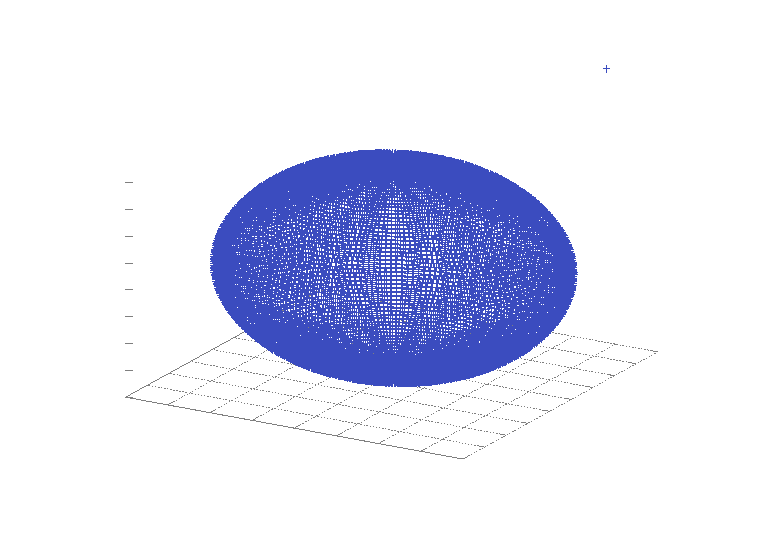
\includegraphics{tested_positions}}%
    \gplfronttext
  \end{picture}%
\endgroup

  \caption{Visualisierung der getesteten Positionen}
  \label{fig:pos}
\end{figure}
Für jeden getesteten Radius haben wir Punkte auf der Kugeloberfläche in 2° Auflösung, also insgesamt 32400 Positionen, getestet.
\begin{figure}[H]
  \centering
  \input{img/pos_sweep}
  \caption{Genauigkeit für verschiedene Abstände}
  \label{fig:pos_sweep}
\end{figure}
Bei einem Radius von $0.25m$ gibt es einen Ausreißer mit $3.97743^\circ \pm 0.387624^\circ$, da sich die Positionen innerhalb des Tetraeders befinden. Bis $1.75m$ bleibt die Abweichung deutlich unter $2^\circ$, ist also deutlich besser als beim Menschen. Dieser kann auf sehr kurze Distanzen zwischen $10cm$ und $40cm$ gerade einmal mit $3^\circ$ Genauigkeit die Richtung bestimmen.
Um die Abhängigkeit der Genauigkeit der Richtungsbestimmung von der Frequenz zu untersuchen haben wir die Schallquellen wieder auf einer Kugeloberfläche mit $2^\circ$ Auflösung plaziert und haben anstelle des Radius die Frequenz variiert. Für den Radius haben wir $1.4m$ gewählt.
\begin{figure}[H]
  \centering
  \input{img/freq_sweep}
  \caption{Genauigkeit für verschiedene Frequenzen}
  \label{fig:freq_seep}
\end{figure}
Man sieht, dass die Genauigkeit der Richtungsbestimmung (fast) unabhängig von der Frequenz der Schallquelle ist. Für Frequenzen über $675Hz$ ist die Bedingungen, dass die Abstände der Mikrofone kleiner als die halbe Wellenlänge sein muss nichtmehr erfüllt ist.
\subsection{Praxis}
In unseren Simulationen hat sich gezeigt, dass unser Verfahren theoretisch relativ genau arbeitet. Um die Genauigkeit in der Echtwelt zu untersuchen haben für acht verschiedene Positionen der Schallquelle die Abweichung der Richtung bestimmt. Diese Messung haben wir in einem mit speziellem Schaumstoff~\cite{basotect} ausgekleideten Raum durchgeführt, um Störungen wie Reflektionen zu minimieren. Der Lautsprecher war jeweils $0.75m$ von dem Zentrum der Mikrofone entfernt.
\begin{figure}[H]
  \centering
  \input{img/real}
  \caption{Genauigkeit in der Echtwelt}
  \label{fig:real}
\end{figure}
Für die acht verschiedenen Richtungen hatte die Richtungsbestimmung eine Genauigkeit von $3.9^\circ \pm 0.13^\circ$. Allerdings hatte der Lautsprecher bei dem von uns gewählten Abstand eine Größe von $3.2^\circ$, genauer also diese kann die Richtungsbestimmung also nicht sein. Die Richtungsbestimmung mit unserem Verfahren ist also auch in der Echtwelt genauer als der Mensch.